\section{Uppgift 3}\label{uppgift-3}

\subsection{Instruktioner}
\begin{verbatim}
3. Skriv ett program som räknar om mil till kilometer. Användaren ska mata in
   antal mil som ett decimaltal. Sedan ska programmet konvertera till kilometer
   och skriva ut hur många kilometer det blev. Exempel på utskrift, användarens
   inmatning är markerat med fetstil/understrykning:

    Program som konverterar mil till km.
    Skriv in antal mil: *35.4*
    Motsvarande antal km: 354
\end{verbatim}

\subsection{Lösning}
\subsubsection{Kommentar}
Det enda anmärkningsvärda här är hur texten skrivs ut med
\texttt{System.out.format()} för att få finare kontroll över formatteringen.
Inkluderat i kommentarerna på raderna \numrange{28}{34} är delar av
dokumentationen från Oracle
\footnote{\url{https://docs.oracle.com/javase/tutorial/java/data/numberformat.html}}
på de funktionerna i biblioteket (paketet) som använts.


\subsubsection{Källkod}\label{uppgift-3_src}
%\begin{listing}[H]
    \inputminted[linenos]{java}{src/Lab1Uppg03.java}
    \caption{Lab1Uppg03.java}
    \label{Uppg3src}
%\end{listing}

\subsubsection{Skärmdump}
\begin{figure}[htbp]
    \centering
        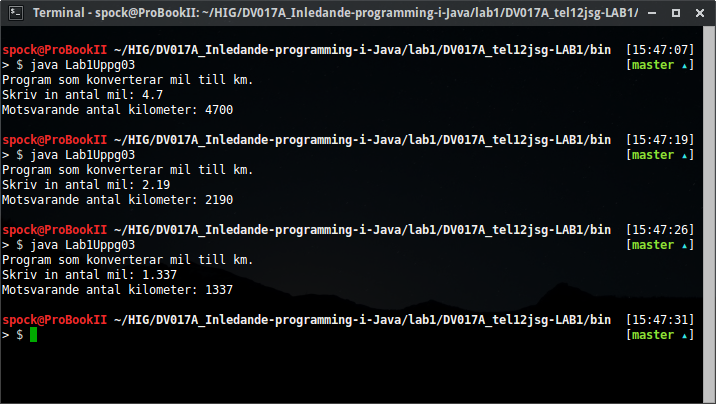
\includegraphics[width=\linewidth]{img/03.png}
    \caption{Körning av koden till Uppgift \ref{uppgift-1}}
    \label{fig:screenshot-03}
\end{figure}
